\chapter{Digital Twin Methodology}\label{ch:ch2}

To design dynamic mirroring based on DT architecture, which anticipates processes in future power system operation, the DT definition and main components that organize synchronization of digital model with physical entity should be introduced. After, a future proof DDM architecture is outlined.

\section{Digital Twin Definition}\label{sec:ch2/sec1}

Digital twin is defined as \emph{a live digital coupling of the state of a physical asset or process to a virtual representation with a functional output} \autocite{jrn_catapult_2021}, originated in the aerospace and aviation industries. However, since that, it has been applied to a wide range of other sectors, including manufacturing  \autocite{conf_moller_2021}, petrochemicals \autocite{jrn_sircar_2023}, automotive \autocite{conf_biesinger_2019}, transportation \autocite{conf_gao_2021}, retail \autocite{conf_maizi_2019}, logistics \autocite{jrn_abideen_2021}, smart cities \autocite{jrn_wang_2023} and healthcare \autocite{jrn_mihai_2022}. The vast amount of capabilities of DT technology allows for effective boosts in the aforementioned sectors and the power energy sector is not excluded \autocite{jrn_bazmohammadi_2022}. %A review of the industrial applications of digital twins can be found in\autocite{jrn_tao_2018}. 

Figure~\cref{fig:dt_definition} illustrates the connection between the physical system comprising the processes and components of a microgrid and its digital twin, as well as the data exchange that is transferred between these two systems.

\begin{figure*}[htbp]
    \centering
    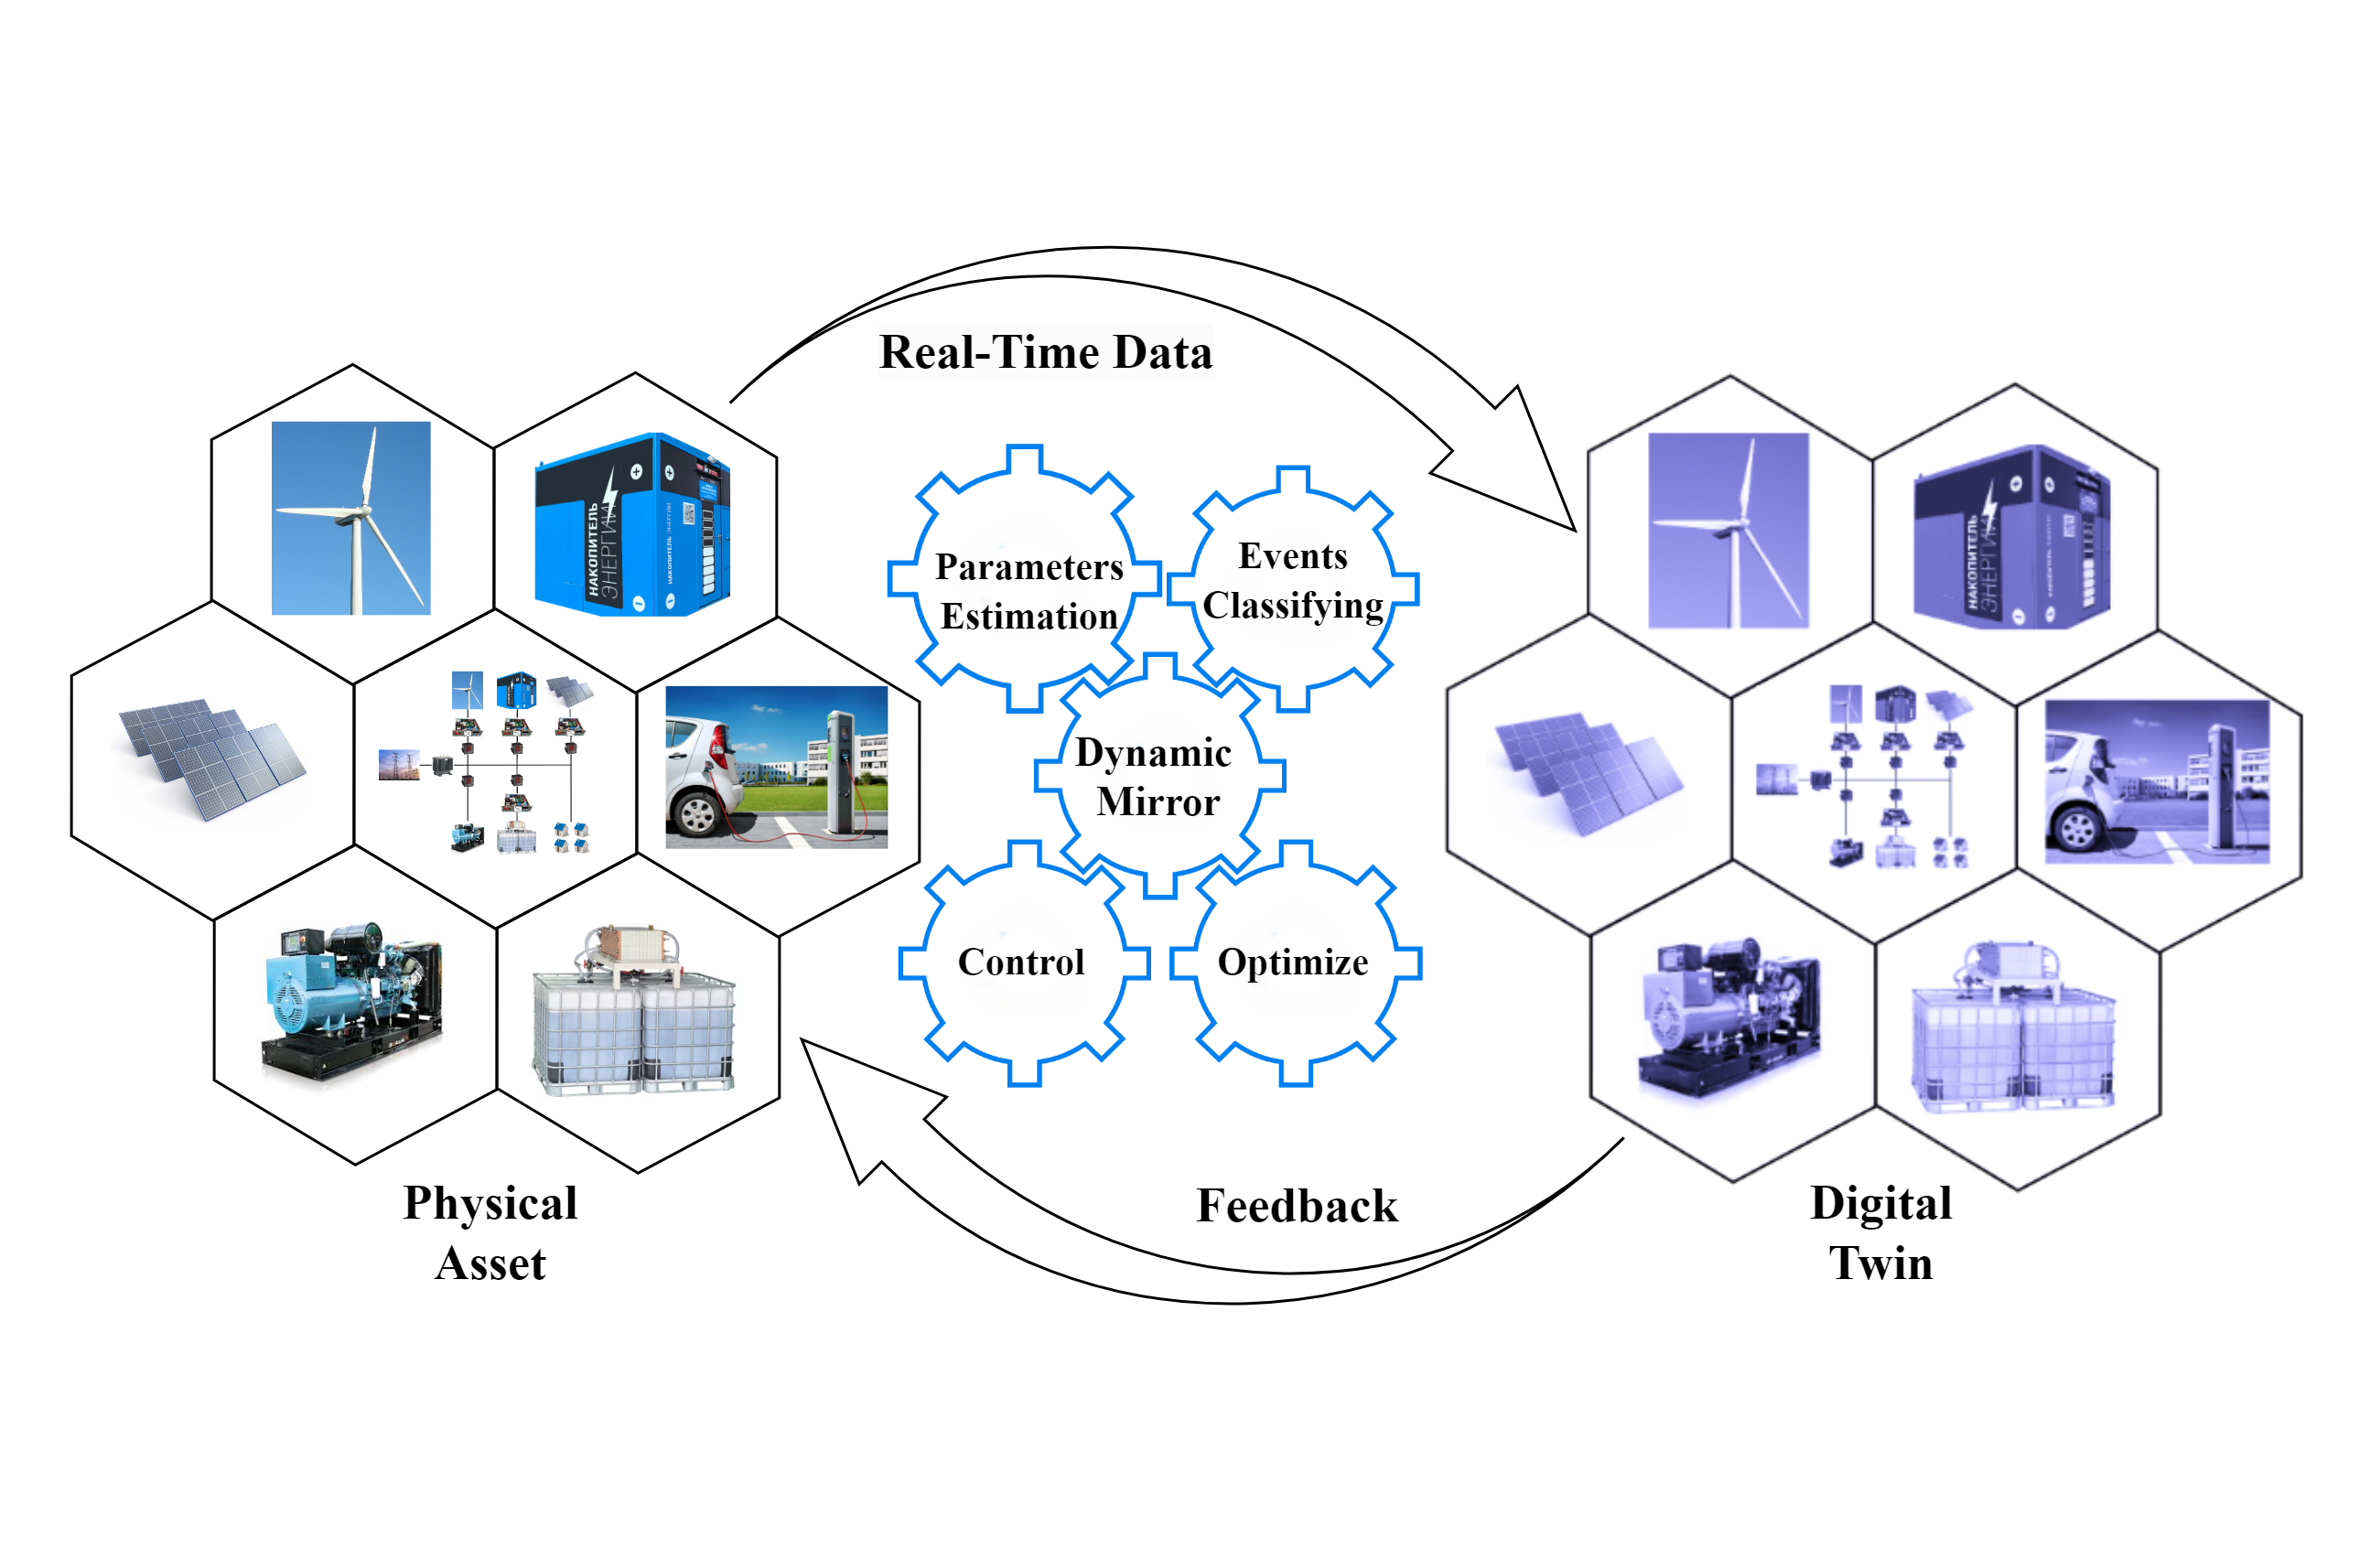
\includegraphics[width = 1\textwidth]{dt_def2.png}
    \caption{Simplified illustration of digital twin definition.}
    \label{fig:dt_definition}
\end{figure*}

The DT approach incorporates three important parts: physical system, virtual system and the data exchange between these two systems. Depending on the level of interaction for these entities, the following definition classification can be applied \autocite{9103025} and shown in Figure~\cref{fig:dt_type}:

\textit{Digital model}: is a digital version of a physical system without automatic data exchange. Changes in the physical or logical object do not affect each other once the model is made.

\textit{Digital shadow}: is a digital representation of a physical system where data flows only from the physical to the digital side. Any change in the physical item's state affects the digital representation, but not vice versa.

\textit{Digital twin}: is a two-way integrated data exchange between a physical object and its digital counterpart, where alterations in one trigger changes in the other automatically.

\begin{figure*}[htbp]
    \centering
    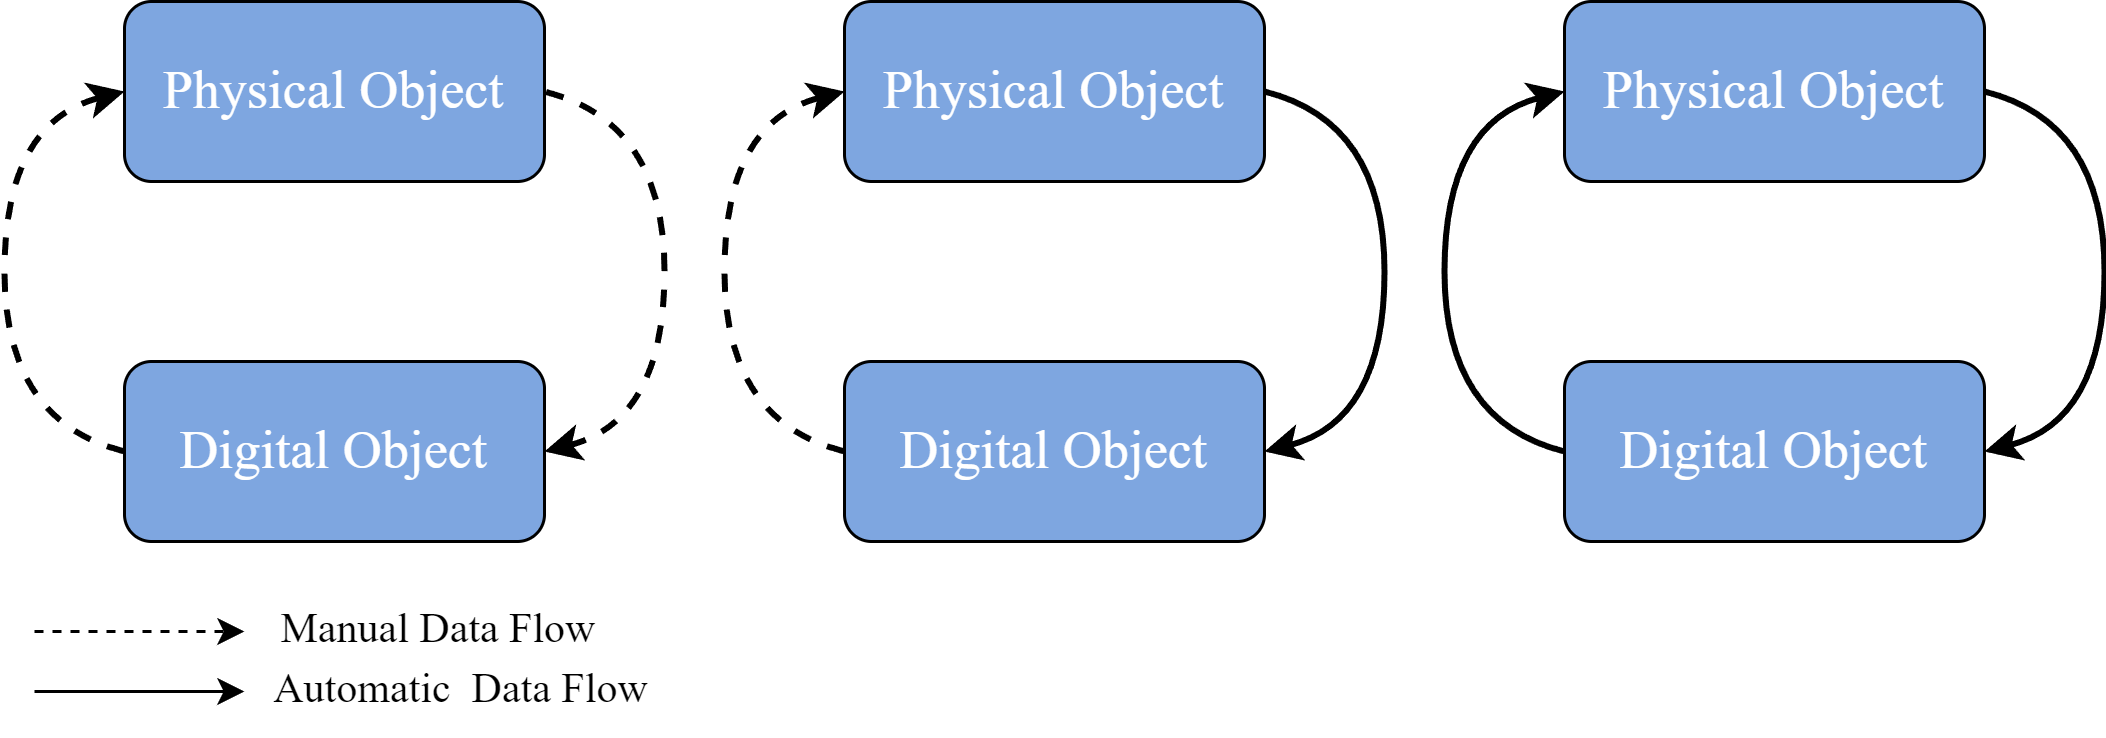
\includegraphics[width=1\textwidth]{dt_type.png}
    \caption{Digital twin definition classification.}
    \label{fig:dt_type}
\end{figure*}

As can be seen from the schematic view in Figure~\cref{fig:dt_type}, the main difference between a digital model and a DT is the ability to exchange data bidirectional with the physical object automatically. The extended comparison of DT characteristics with conventional simulation are presented in Table \ref{tab:dt_vs_sim}.

% Requires: \usepackage{array}
\begin{table}[h]
    \centering
    \caption{Conventional Simulation and Digital Twin comparison}
    \begin{tabular}{|>{\centering\arraybackslash}m{3.4cm}|>{\centering\arraybackslash}m{5cm}|>{\centering\arraybackslash}m{5cm}|}
    \hline
    \textbf{Feature} & \textbf{Conventional simulation} & \textbf{Digital Twin} \\ \hline
    Communication & One-way or no communication with the simulation & Two-way, automated, closed-loop interaction \\ \hline
    Speed & No real-time constraints & Designed for real-time processing \\ \hline
    Data Scope & Limited to scenario-specific inputs & Captures full lifecycle data \\ \hline
    Modeling approach & Pure data-driven or physics-based models & Hybrid: integrates physics and data-driven approaches \\ \hline
    \end{tabular}
    % \caption{Comparison of Conventional Simulation and Digital Twin Features}
    \label{tab:dt_vs_sim}
\end{table}

A model for a DT should be physics-based, accurate enough, and ideally in real time \autocite{Wright_Davidson_2020, VANDERHORN2021113524}. Thus, DT serves as a digital model that analytically evaluates the discrete-time states of physical systems. Analytical models suggest that DT can infer unobservable state values and relay them to the physical world. This core attribute of DT appears to the observer concept commonly used in control engineering, where mathematical model of the original system and a function of the measurement noise (i.e., a correction term) apply to estimate the system state from measurements \autocite{simon2006optimal}. 

The fundamental idea of the DT methodology is depicted in Figure~\cref{fig:dt_generic}. Depending on the specific DT model employed, the input signal $u^m$, the observed output $y^m$, and the predicted response of the model $\hat{y}^{DT}$ are presented in a general form, which can consist of singular or multiple values. If the observed output $y^m$ does not align with the model's response $\hat{y}^{DT}$ when using identical independent input variables $u^m$, it indicates inaccuracies in the formulation and structure of the model, necessitating an appropriate method for model parameter identification to achieve a valid model response \autocite{BROSINSKY202379}.

\begin{figure*}[htbp]
    \centering
    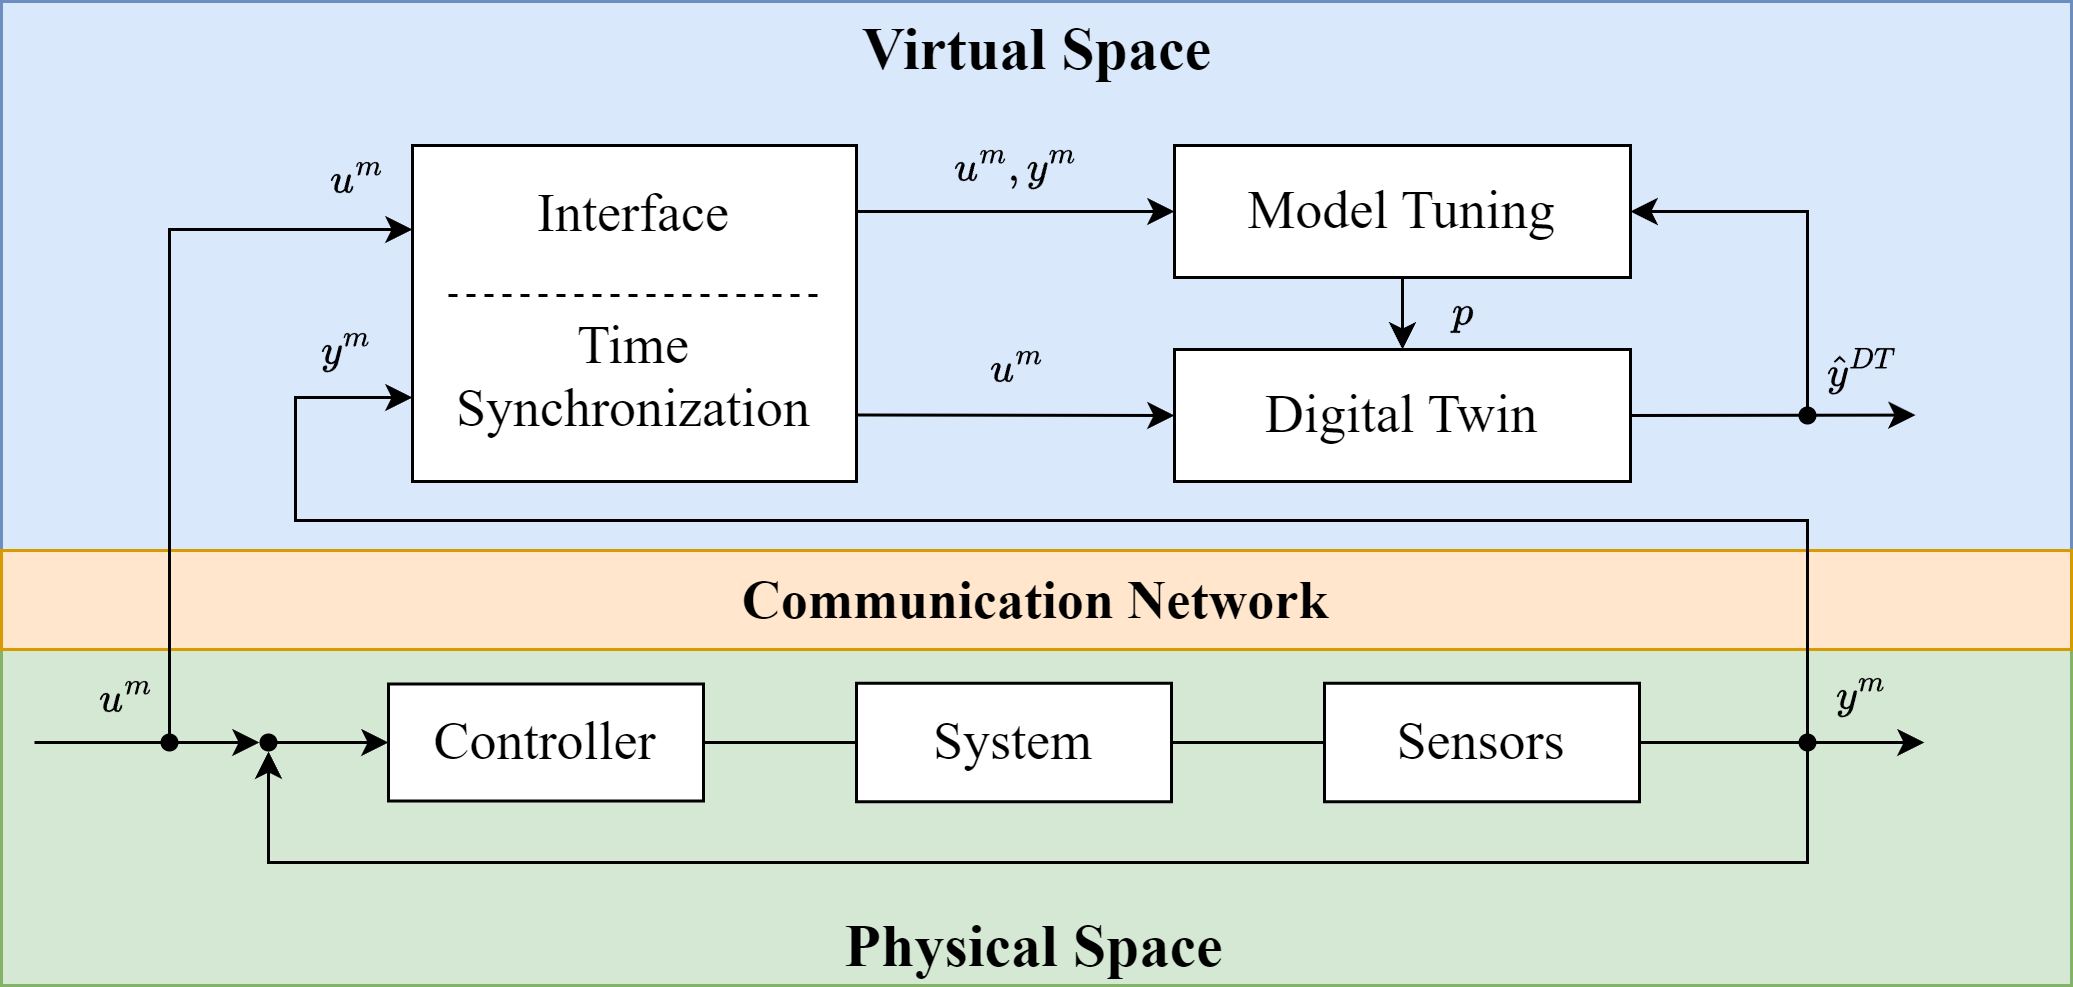
\includegraphics[width=1\textwidth]{generic_dt.png}
    \caption{Simplified generic view of DT.}
    \label{fig:dt_generic}
\end{figure*}

Representing a special form of an observer, DT provides intensive data, which can be effectively utilized for future power system operation. One factor that sets the proposed DT-based concept apart from the traditional observer approach is its greater flexibility regarding the model basis. While the observer is limited to reproducing specific states of a system for the purpose of control, a DT extends this capability by simulating the system's behavior proactively, taking into account alterations in system topology and conditions. 

\section{Model Parameter Identification}\label{sec:ch2/sec2}
To achieve a valid model response a correspondence between the physical object and the parameters of the DT model must be established. This can essentially be achieved through preliminary manual specification or through appropriate method for model parameter identification. Relevant aspects for the selection of a suitable parameter estimation method applicable for time-domain power system models are discussed in the following subsection.

\subsection{Digital Twin Model Types}\label{subsec:ch2/sec2/sub1}

In digital twin simulations, models aim to emulate physical systems accurately enough to provide insights, without becoming too complex or computationally demanding \autocite{10666929, DIZ2023120606}. Achieving the right balance between model accuracy and computational efficiency is vital, as excessive detail can lead to impractical simulation delays, while too simplified models may not deliver the desired insights \autocite{10666932}.

Dynamic systems are typically represented by discrete-time models, which accurately emulate the behavior of the physical system \autocite{WANG2022124, DIZ2023120606}. Depending on the level of prior knowledge about the system, DT models can be categorized into three color-coded levels: \textit{White-box}, \textit{Grey-box} and \textit{Black-box} models as shown in Figure~\cref{fig:dt_models_type} \autocite{Vu2015}. 

\begin{figure*}[htbp]
    \centering
    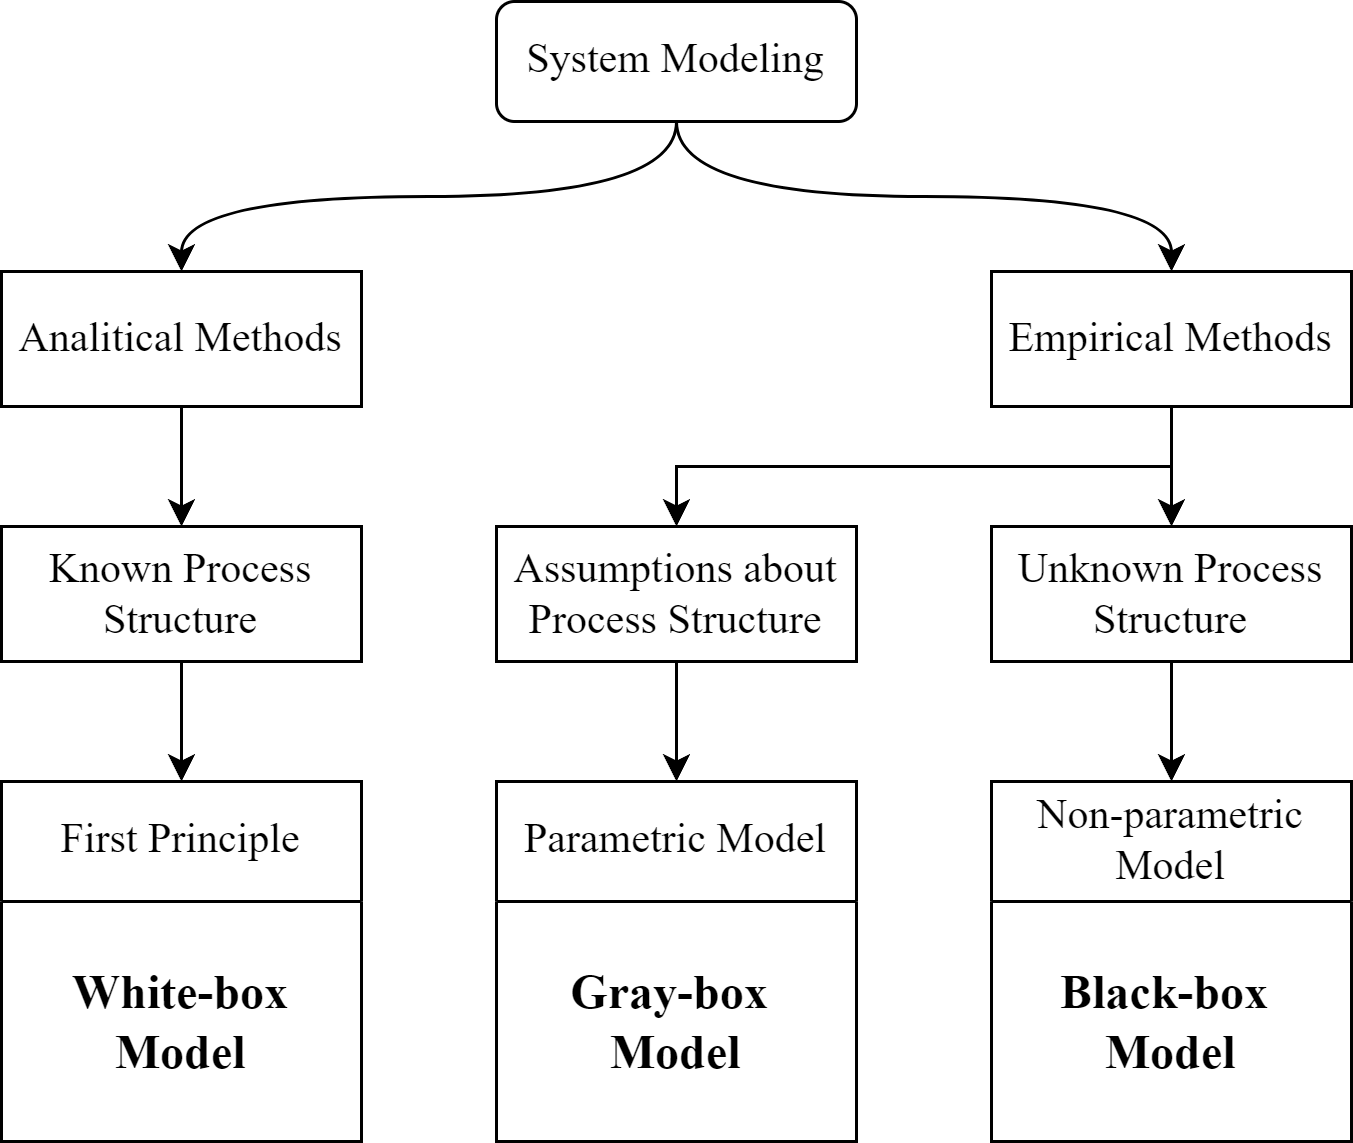
\includegraphics[width=0.75\linewidth]{dt_models_type2.png}
    \caption{Block diagram of DT system modeling approaches.}
    \label{fig:dt_models_type}
\end{figure*}

\textbf{White-box} models, also known as physics-based models, are founded on first principles and exact mathematical equations that describe the system's dynamics, with parameters often directly corresponding to physical attributes. These models require a deep understanding of the system's structure and are known for their high accuracy, which makes them beneficial for precise analysis. However, a significant drawback of white-box models is the substantial effort and high computational burden required for their development and assessment, particularly for complex systems, which can limit real-time applications and scalability.

\textbf{Black-box} is a type of system model where the internal physical structure of the system being modeled is entirely unknown. These models do not allow for direct physical interpretation of their parameters and avoid extensive description by mathematical equations that would represent the internal relations. Instead, they primarily reproduce the input-output behavior of the system, relying solely on empirically obtained data or transfer functions derived from measurements. While flexible, a key disadvantage is their difficulty in scalability and extrapolation, and they do not require expert knowledge or experience for their development as the structure and parameters are derived entirely from measured data.

\textbf{Grey-box} model is a type of system model that combines characteristics of both white-box (known structure and parameters) and black-box (unknown structure and parameters) models. In a grey-box model, the physical structure of the system being modeled is known or assumed, and can often be expressed by equations. However, some or several of the model's parameters are unknown and must be estimated, typically by observation or measurements.

Based on the characterization of the above model system approaches, the summaries are presented in the form of Table \ref{tab:model-types}. As can be seen from table, grey-box offers major adaptability, acting as a versatile model for simulating and deriving system behavior rules. Grey-box models are extensively utilized in model-based control and simulation, making them ideal for dynamic systems modeling in DT.

% Please add the following required packages to your document preamble:
% \usepackage{multirow}
% \usepackage{graphicx}
% \usepackage[table,xcdraw]{xcolor}
% Beamer presentation requires \usepackage{colortbl} instead of \usepackage[table,xcdraw]{xcolor}
\begin{table}[]
\centering
\caption{Model types comparison}
\label{tab:model-types}
\resizebox{\textwidth}{!}{%
\begin{tabular}{|
>{\columncolor[HTML]{EFEFEF}}l |ccc|}
\hline
\multicolumn{1}{|c|}{\cellcolor[HTML]{C0C0C0}} &
  \multicolumn{3}{c|}{\cellcolor[HTML]{C0C0C0}\textbf{Model Type}} \\ \cline{2-4} 
\multicolumn{1}{|c|}{\multirow{-2}{*}{\cellcolor[HTML]{C0C0C0}\textbf{Feature}}} &
  \multicolumn{1}{c|}{\cellcolor[HTML]{C0C0C0}\textbf{White-Box}} &
  \multicolumn{1}{c|}{\cellcolor[HTML]{C0C0C0}\textbf{Grey-Box}} &
  \cellcolor[HTML]{C0C0C0}\textbf{Black-Box} \\ \hline
\begin{tabular}[c]{@{}l@{}}Core \\ Principle\end{tabular} &
  \multicolumn{1}{c|}{\begin{tabular}[c]{@{}c@{}}A model based entirely\\ on well-understood \\ first principles and \\ physical laws.\end{tabular}} &
  \multicolumn{1}{c|}{\begin{tabular}[c]{@{}c@{}}A hybrid model \\ combining a known \\ physical structure with \\ parameters estimated \\ from data.\end{tabular}} &
  \begin{tabular}[c]{@{}c@{}}A data-driven model \\ that maps inputs to outputs \\ without knowledge of the \\ system's internal workings.\end{tabular} \\ \hline
\begin{tabular}[c]{@{}l@{}}System \\ Knowledge\end{tabular} &
  \multicolumn{1}{c|}{\begin{tabular}[c]{@{}c@{}}Structure: Known; \\ Parameters: Known\end{tabular}} &
  \multicolumn{1}{c|}{\begin{tabular}[c]{@{}c@{}}Structure: Known; \\ Parameters: Unknown;\end{tabular}} &
  \begin{tabular}[c]{@{}c@{}}Structure: Unknown; \\ Parameters: Derived \\ from data;\end{tabular} \\ \hline
\begin{tabular}[c]{@{}l@{}}Development \\ Basis\end{tabular} &
  \multicolumn{1}{c|}{\begin{tabular}[c]{@{}c@{}}Theoretical knowledge and \\ mathematical equations.\end{tabular}} &
  \multicolumn{1}{c|}{\begin{tabular}[c]{@{}c@{}}A combination of known \\ physical laws and \\ experimental \\ measurement data.\end{tabular}} &
  \begin{tabular}[c]{@{}c@{}}Exclusively experimental \\ data and statistical fitting.\end{tabular} \\ \hline
Advantages &
  \multicolumn{1}{c|}{\begin{tabular}[c]{@{}c@{}}Highly accurate and \\ physically interpretable.\\ Transparent and easy \\ to understand.\end{tabular}} &
  \multicolumn{1}{c|}{\begin{tabular}[c]{@{}c@{}}Balances physical insight \\ with real-world data.\end{tabular}} &
  \begin{tabular}[c]{@{}c@{}}Does not require \\ deep expert \\ domain knowledge.\end{tabular} \\ \hline
\begin{tabular}[c]{@{}l@{}}Disadvantages  \\ Requirements\end{tabular} &
  \multicolumn{1}{c|}{\begin{tabular}[c]{@{}c@{}}Requires deep expert \\ knowledge and experience.\\ Very difficult and \\ time-consuming to \\ develop for large or \\ complex systems.\end{tabular}} &
  \multicolumn{1}{c|}{\begin{tabular}[c]{@{}c@{}}Requires access \\ to the system \\ for measurements. \\ Model accuracy \\ depends on \\ the quality of \\ measurement data.\end{tabular}} &
  \begin{tabular}[c]{@{}c@{}}Lacks physical \\ interpretability. \\ Poor at extrapolating \\ beyond the training data. \\ Can lack flexibility \\ and scalability.\end{tabular} \\ \hline
\end{tabular}%
}
\end{table}

% As grey-box and black-box models arise from parametric and non-parametric models, two general model identification methods can be distinguished. Non-parametric identification fits a broad model to time-domain or frequency spectrum data, whereas parametric identification employs optimal search methods to align the model parameters with those of the real system by minimizing output deviations \autocite{4111713}. Given the known model structure for DT applications, we focus on algorithms that minimize the gaps between measured and simulated results using an error function. With the choice of parametric grey-box models, we assess procedures tailored for the parameter estimation of these models.

Model-based optimization and control strategies require precise models. Achieving accuracy in power systems modeling requires knowledge of both the model's structure and its parameters. Although the detailed topology of transmission systems at most voltage levels is well documented, the focus remains on identifying the parameters of the system model. To keep the model up-to-date, an online parameter estimation method is essential. Thus, a robust methodology, capable to estimate parameters of linear and nonlinear models is therefore proposed in the following subsection.


\subsection{Parameter Estimation}\label{subsec:ch2/sec2/sub2}

The efficiency of DT is fundamentally based on its ability to accurately reflect the phenomena of the physical power system \autocite{Song2019}. However, knowledge about parameters is often limited or may change during operation due to factors such as saturation effects, temperature variations, weather conditions and aging \autocite{10615087}. To close this gap, an adaptive parameter tuning algorithm involved to continuously updates the DT model using incoming real-time data, as it shown in Figure~\cref{fig:sch_estimation}. This scheme illustrates the complete workflow of parameter estimation and how it maintains alignment between the digital twin and its corresponding physical power grid. The process begins with collecting measurement data—typically using devices like PMUs, IEDs or RTUs. These measurements are transmitted via communication protocols to a centralized database, to which DT interfaces through a simulation platform.

\begin{figure*}[htbp]
    \centering
    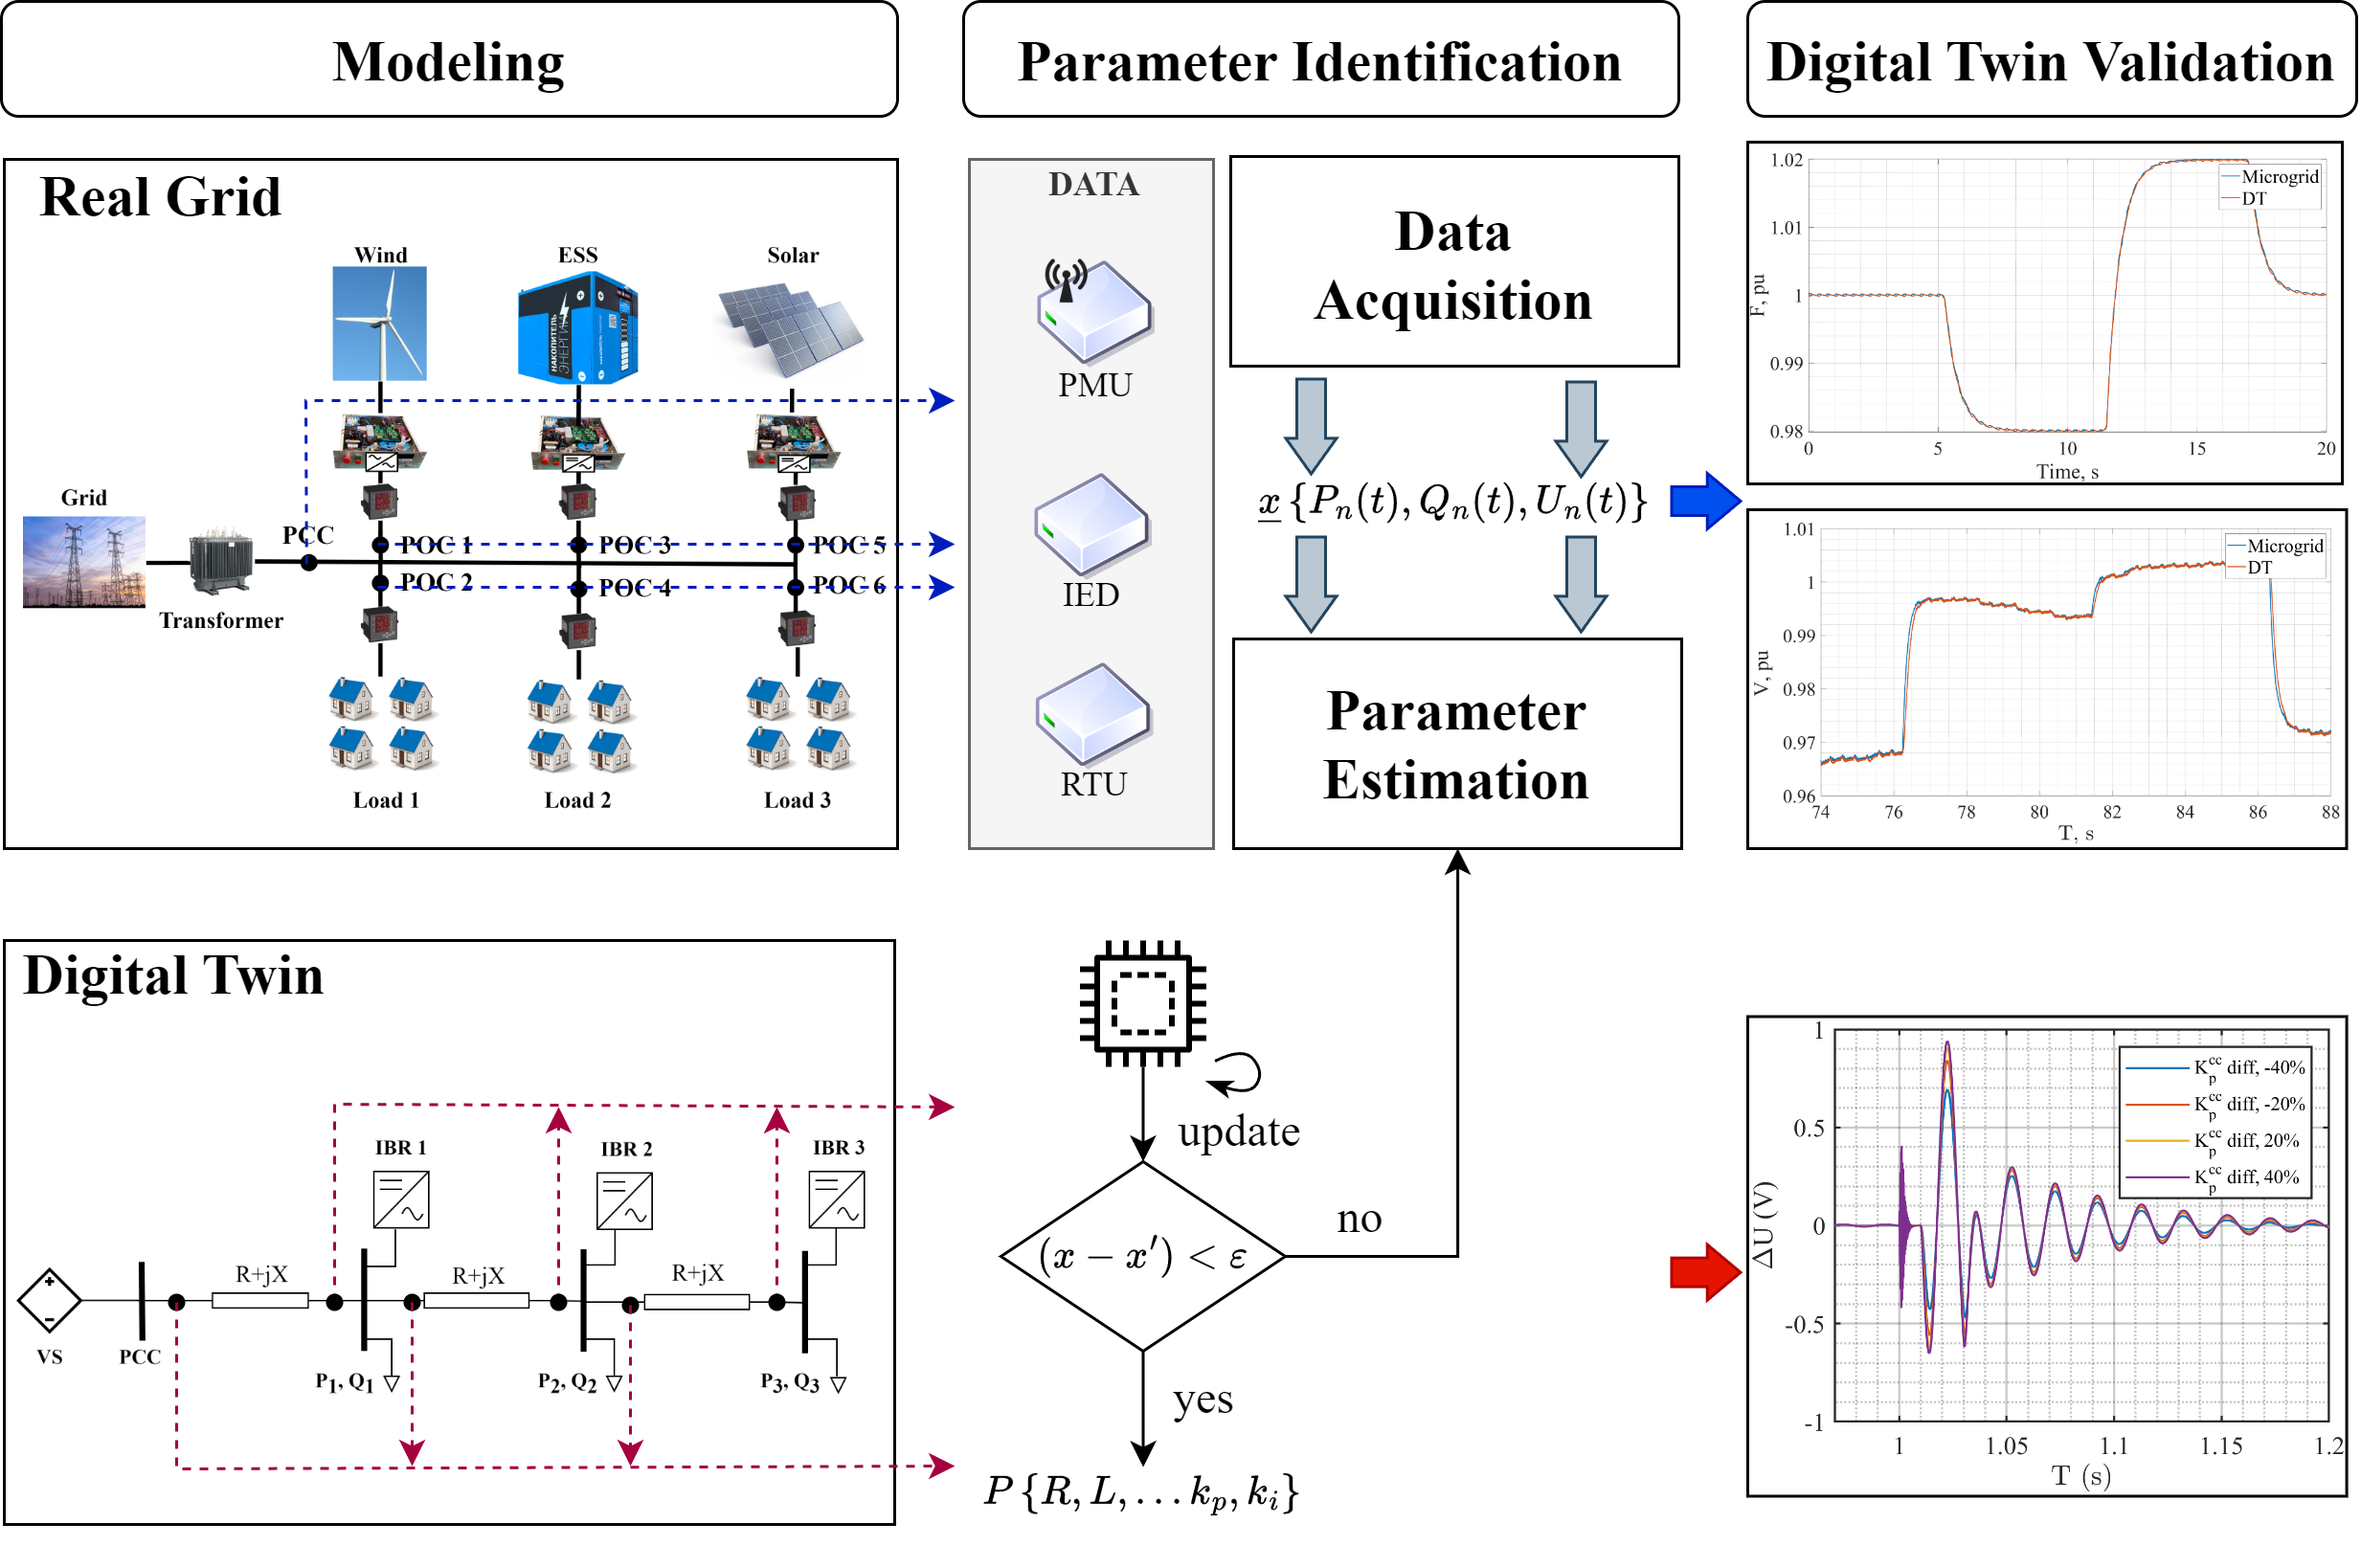
\includegraphics[width=1\linewidth]{sch_estimation.png}
    \caption{Digital twin parameter identification schematic}
    \label{fig:sch_estimation}
\end{figure*}

Parameter estimation aims to compute coefficients in DAEs that align with the measurement vector by minimizing an objective function. The main four steps in the parameter estimation task shown in Figure~\cref{fig:dgm_estimation} and include \autocite{Vu2015}: 

\begin{enumerate}

    \item \textbf{Model (re)formulation} step involves constructing a mathematical model based on prior physical understanding with unknown parameters.
    
    \item \textbf{Parameter estimation} step uses optimization techniques to minimize the difference between measured data and model outputs, yielding one or more parameter sets.
    
    \item \textbf{Model validation} stage assesses the quality of the estimation phase. Validation data must be gathered independently from the estimation data. The key question here is whether the parameter set estimated is unique, addressing the identifiability problem. A model is identifiable if it has a unique parameter solution; otherwise, it is non-identifiable, rendering it unreliable. Identifiability has two types: structural and practical. Structural identifiability is verified using ideal noise-free data, reflecting the model's inherent properties, and should be assessed prior to experiments. However, it alone doesn't guarantee accurate parameter estimation from real data. Practical identifiability pertains to real, noisy measurements and depends on experimental execution, resolvable through careful experiment design.
    
    \item \textbf{Experimental design} generates real measurement data, but its quality can be influenced by input signals, sensor setup, and test conditions. Data must be preprocessed before parameter estimation, and due to practical identifiability issues, this step may need to be repeated to achieve a reliable parameter set. 
    
\end{enumerate}

\begin{figure*}[htbp]
    \centering
    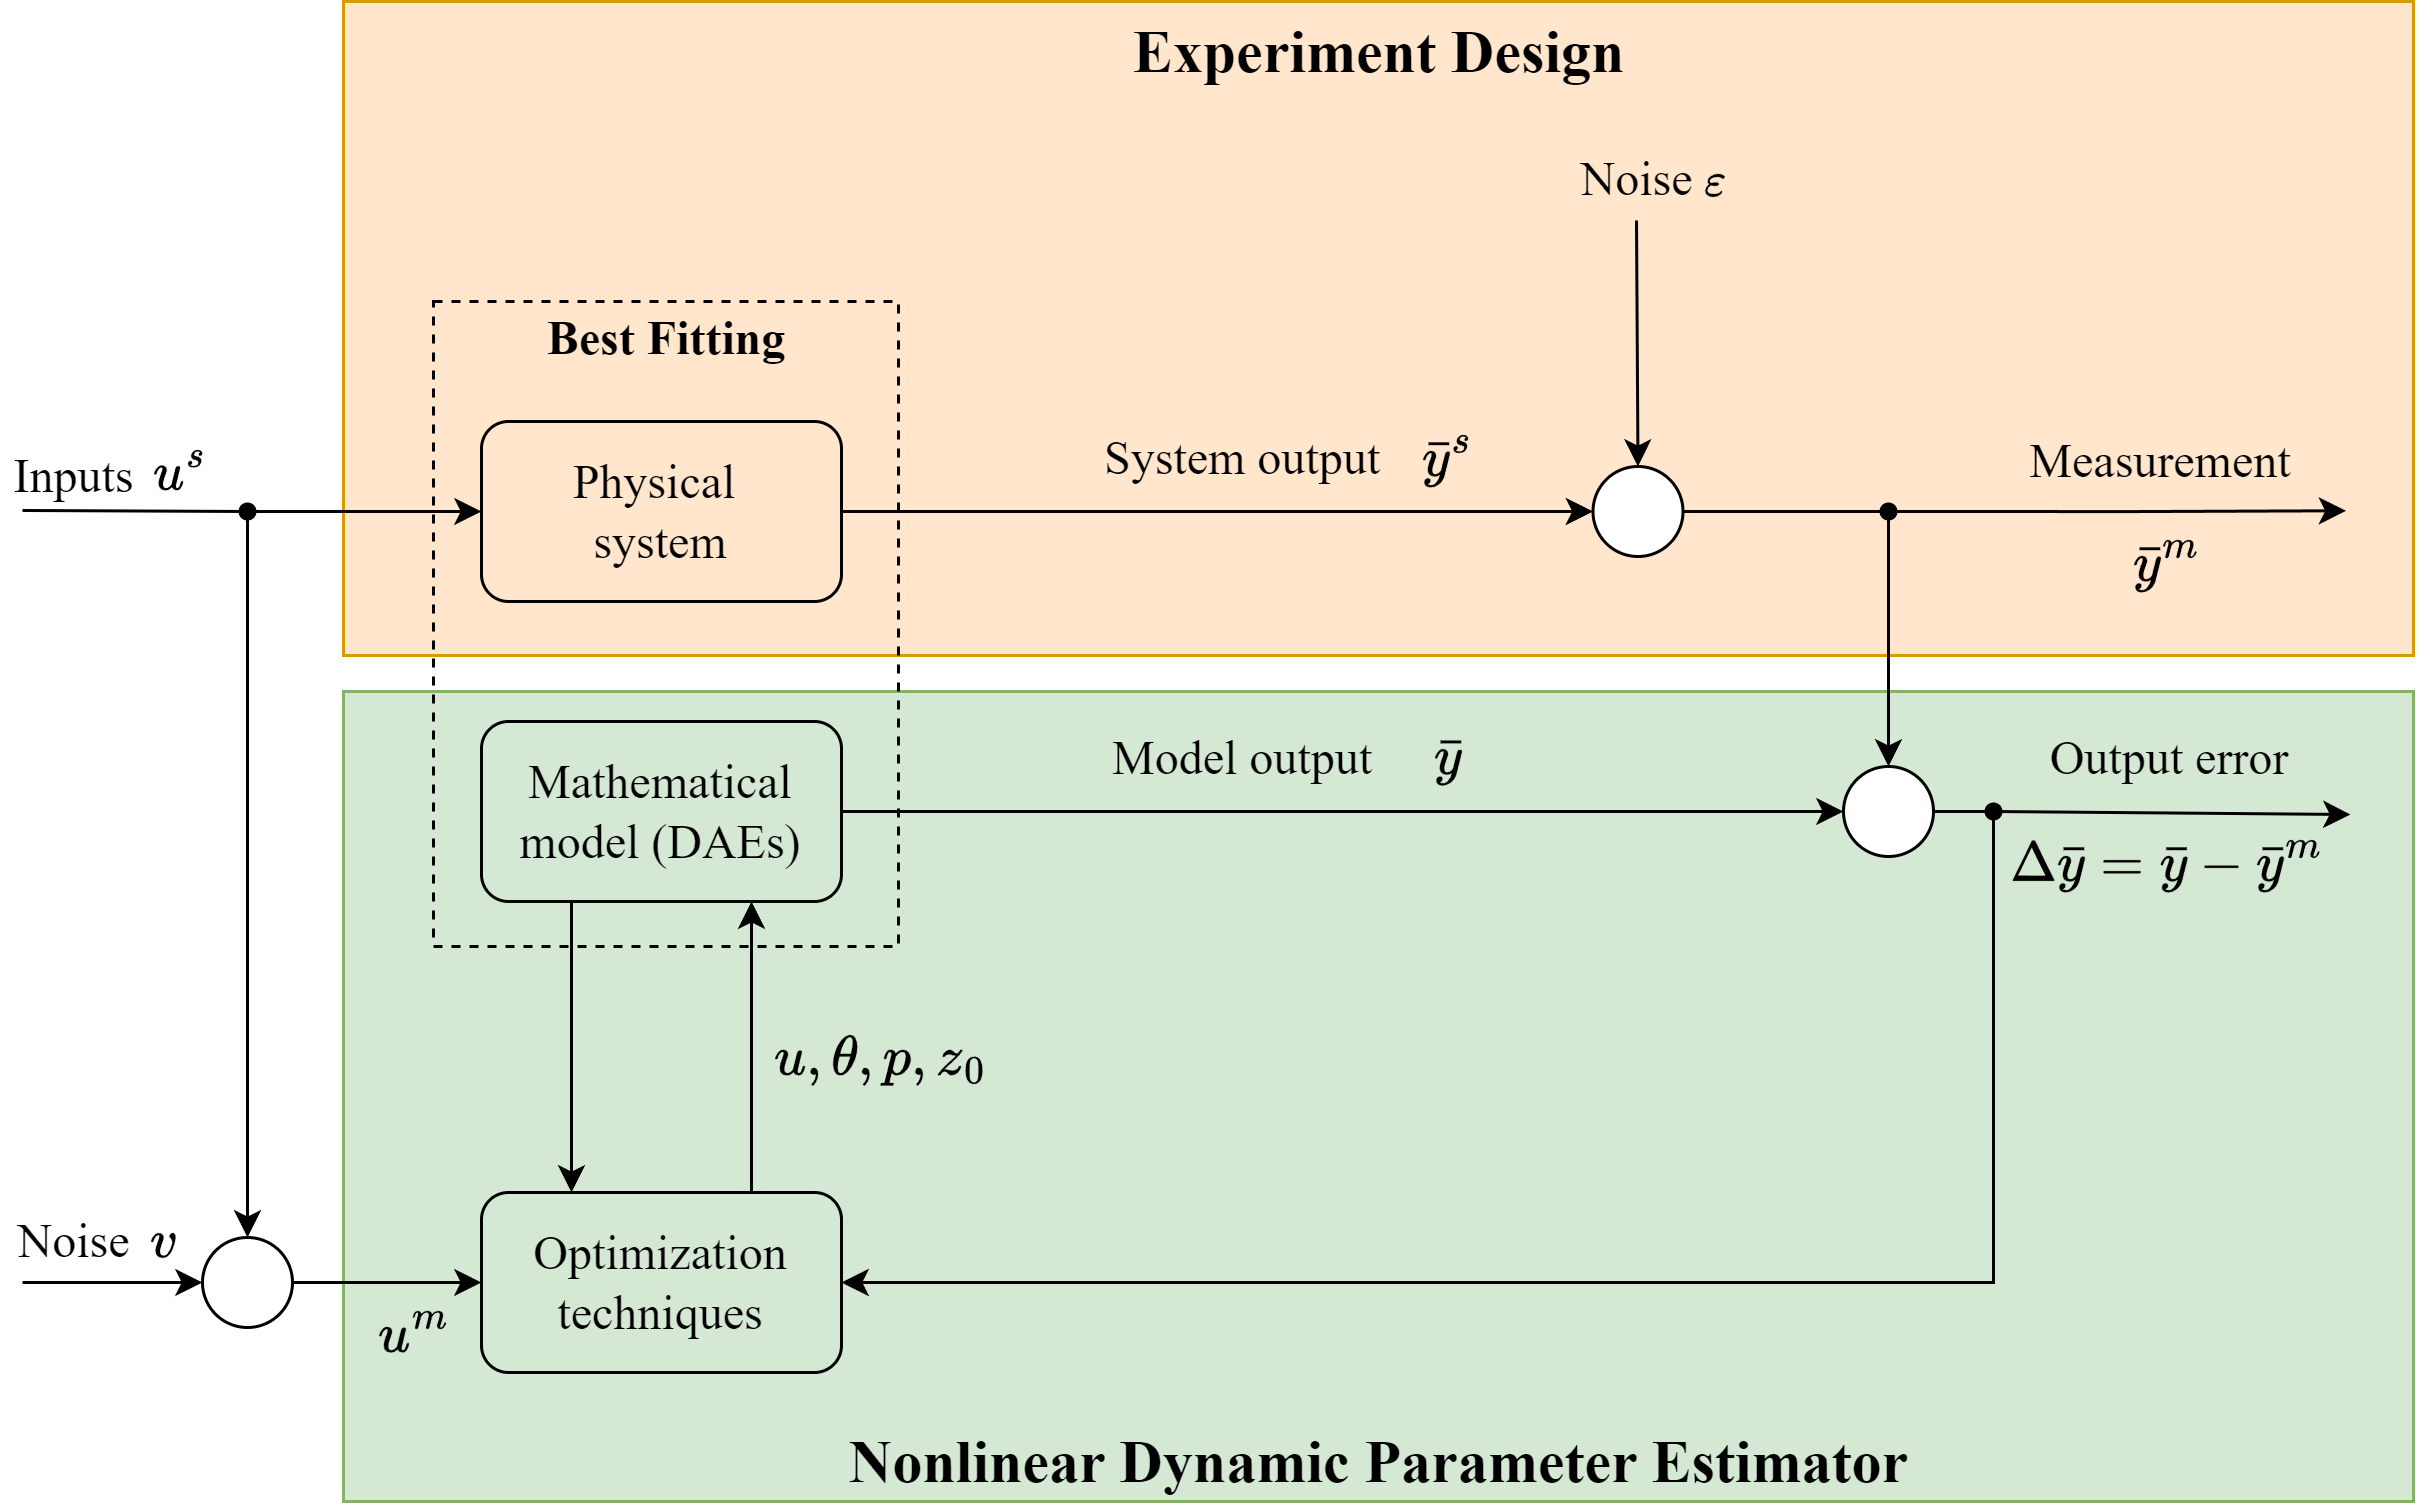
\includegraphics[width=1\linewidth]{dgm_estimation.png}
    \caption{Diagram of the DAEs system parameter estimation procedure.}
    \label{fig:dgm_estimation}
\end{figure*}

The idea of parameter estimation to calculate the coefficients in DAEs to fit the measurement vector. It is usually done by minimizing a scalar function called objective function that includes the difference or residuals $\boldsymbol{e}_i$ between input-output of the DT and the measured data [35, 63]:

\begin{equation}
    \varepsilon_i=\left|x_i^m-x_i\right|
\end{equation}

where $x=[\overline{\boldsymbol{y}} \boldsymbol{u}]^{\mathrm{T}}$ and $x^m$ represents the measurement. $\overline{\boldsymbol{y}}$ is the output calculated with the estimated parameters, and $\boldsymbol{u}$ is the input data vector. 

An application of the above technique can be the estimation of transmission line parameters, where data from PMU and SCADA measurements are involved along with \autocite{PEGORARO2023113175, Albuquerque2021, JYang2010, 7465793, 7807323, 9494814}. The authors estimate the full nodal admittance matrix $Y_{bus}$ applying the weighted least squares and the extended Kalman filter (EKF). In addition, the Kalman filter and its derivatives, such as the EKF and the UKF or the cubature Kalman filter, successfully applied by researchers in DSE techniques for system model validation and dynamic model parameter calibration \autocite{6420999, 8070959} what helps for wide area control and stability monitoring \autocite{9210125}.

For dynamic modeling in the time-domain, additional attributes are required to model the behavior of rotating machinery, inverters and their respective controllers. In \autocite{9640105}, the state-of-the-art parameter estimation method based on least squares is presented \autocite{dbt_mods_00026727} to develop dynamic models in DT of synchronous generators. The recursive least squares algorithm \autocite{LANDAU2001469} is mentioned in \autocite{conf_song_2020} to parameterize the DT of inverter-based feeds for monitoring the operations of the physical power system.

Parameter estimation techniques using the autoregressive moving average model have been utilized to estimate the parameters of the power plant \autocite{754830} and to assess inertia within the synchronous area \autocite{8370893}. A recent technique estimates power system inertia and equivalent damping of synchronous machines online, including virtual inertia and droop from converter-interfaced generators, by fitting ambient measurement covariance to a synchronous machine model using non-linear least-squares optimization \autocite{10015690}. Another method enables robust on-line tracking of constant and time-varying inertia for both synchronous and non-synchronous devices, along with the fast frequency response droop gain, through improved, numerically stable formulas that account for damping effects \autocite{9253523}. 

The method typically employed for robust parameterization is active parameter estimation using an artificial neural network (ANN) \autocite{1224042}. Current advancements in estimating non-measurable states using ANN can be found in \autocite{Song2019,AhmedAli01082007}, which outline adaptive estimation of controller parameters to develop the inverter DT. This approach focuses on parameter estimation in the continuous time domain for a broad range of unknown parameters. Several authors have introduced hybrid approaches, particularly Physics-informed Neural Networks (PINN), which integrate artificial intelligence with physical principles for accurate modeling and robust parameter estimation \autocite{10567996}. PINNs are noteworthy for their ability to be well-trained with small datasets and without additional hardware circuitry, successfully estimating DC-link capacitance and AC-side inductance parameters for three-phase inverters with satisfactory accuracy. Bayesian Physics-informed Neural Networks (BPINNs) extend PINNs by incorporating Bayesian techniques to quantify uncertainties in data and models, providing a confidence indication that standard PINNs lack \autocite{STOCK2024110860}. BPINNs have shown robustness against noisy data and achieved significantly lower estimation errors compared to conventional methods like sparse identification of nonlinear dynamics and even PINNs, particularly when dealing with model uncertainties from IBRs. Earlier methods for inverter parameter identification include least square system identification and step identification strategies, though these were associated with lower efficiency or larger identification errors.


\section{Digital Twin Based Event Identification}\label{sec:ch2/sec3}

DT operates in real-time alongside the actual power grid, continuously tracking its operational state. When significant discrepancies arise between real-time sensor data and the DT’s predictive state estimations, it may signal abnormalities in the physical system. Anomalous events within a power system refer to unexpected incidents that deviate significantly from the system’s normal operating state \autocite{ASEFI2023101116, ZANG2025110813}. These anomalies may include equipment failures, abrupt shifts in load or generation, or electrical disturbances like short circuits \autocite{Li_2021}. Each of these events leaves a unique signature on the measurement data, allowing their potential identification and allowing operators to respond to unexpected grid behavior promptly. 

The digital twin approach can extensively amplify the identification ability enhanced by ML algorithms, to accurately detect and categorize these anomalies, providing critical insights to assist system operators. The process of recognizing and understanding such events typically follows three sequential steps: detection, classification, and identification \autocite{Chandola2009}.

Event detection involves recognizing the presence of abnormal behavior in system operations \autocite{Chandola2009}. Using real-time measurement data, specific algorithms or rule-based thresholds can indicate the occurrence of a disturbance \autocite{ma2018clsf, 0cba72bc98634e678681cd57ee34bc59, 6465867}. A large body of literature focuses on detecting anomalies using data from PMUs \autocite{ASEFI2023101116, 6345522, 8274161, 10295481, hannon2019anml}. For example, \autocite{6345522, vasiliev2024mle} introduce Maximum Lyapunov Exponent (MLE) as a technique to find stable and unstable modes of power system operation. In stable operating mode MLE is negative, in unstable mode it is positive. The authors in \autocite{8274161, 10295481} evaluate two detection approaches: one using the normalized wavelet energy function, which calculates the RMS of detail coefficients that reflect the nonstationary occurrence of significant changes in signals, and another based on the Hankel alternative view of the Koopman analysis. The method described in \autocite{7511666} applies a linear dynamic system model to detect deviations according to rule-based criteria. In contrast, \autocite{Mampilly2024, 8274161} employs wavelet transformation techniques for detection. In \autocite{8831027cd83c49519d85cab789591467}, various detection methods are explored, such as Fast Fourier Transform, Matrix Pencil Method, Yule-Walker analysis, the Min-Max method and data-driven techniques. These centralized methods produce excessive data, many of which lack relevance. The usefulness of the data is largely influenced by the scale and location of the anomaly. Efficient detection can be achieved by filtering for key data, like representative pilot nodes as in \autocite{8117615,6465867}, utilizing signal processing techniques. The promising solution comes from hybrid methods, where model-based approaches combine with data-driven methods \autocite{ASEFI2023101116}, which allow ML models to work with limited statistical data, improve feature selection, and increase the accuracy of anomaly detection.

Following detection, the next step is to classify the event type and uncover its root cause. The authors in \autocite{7540867} achieved event classification using voltage magnitude and phase angle data, distinguishing between scenarios such as generator trips, load or capacitor switching, short circuits, or disconnection of lines and motors. Ongoing research primarily divides into two main approaches: data-driven (statistical/ML-based) \autocite{biau2015randomforestguidedtour, Hochreiter_1997}, model-based (physics-based) methods \autocite{7511666,4596578} and hybrid methods combining them \autocite{ASEFI2023101116, vasiliev2024mle}.

Data-driven methods rely on comparing real-time data against a precompiled event database. This includes identifying patterns and classifying them using trained models. Direct time-series comparisons are not ideal for high-dimensional data; therefore, feature extraction is necessary to identify relevant characteristics, which are then fed into a classifier. This process is illustrated in Figure~\cref{fig:dt_ml_idnt}. Training data typically includes both historic measurements and dynamic simulations generated via DTs. Several classification algorithms are applied, including those based on signal processing, statistics, and ML (e.g., SVM, kNN, Decision Trees) \autocite{idrisov2025leveragingdigitaltwinmachine}.

\begin{figure}[htbp]
    \centerfloat{
        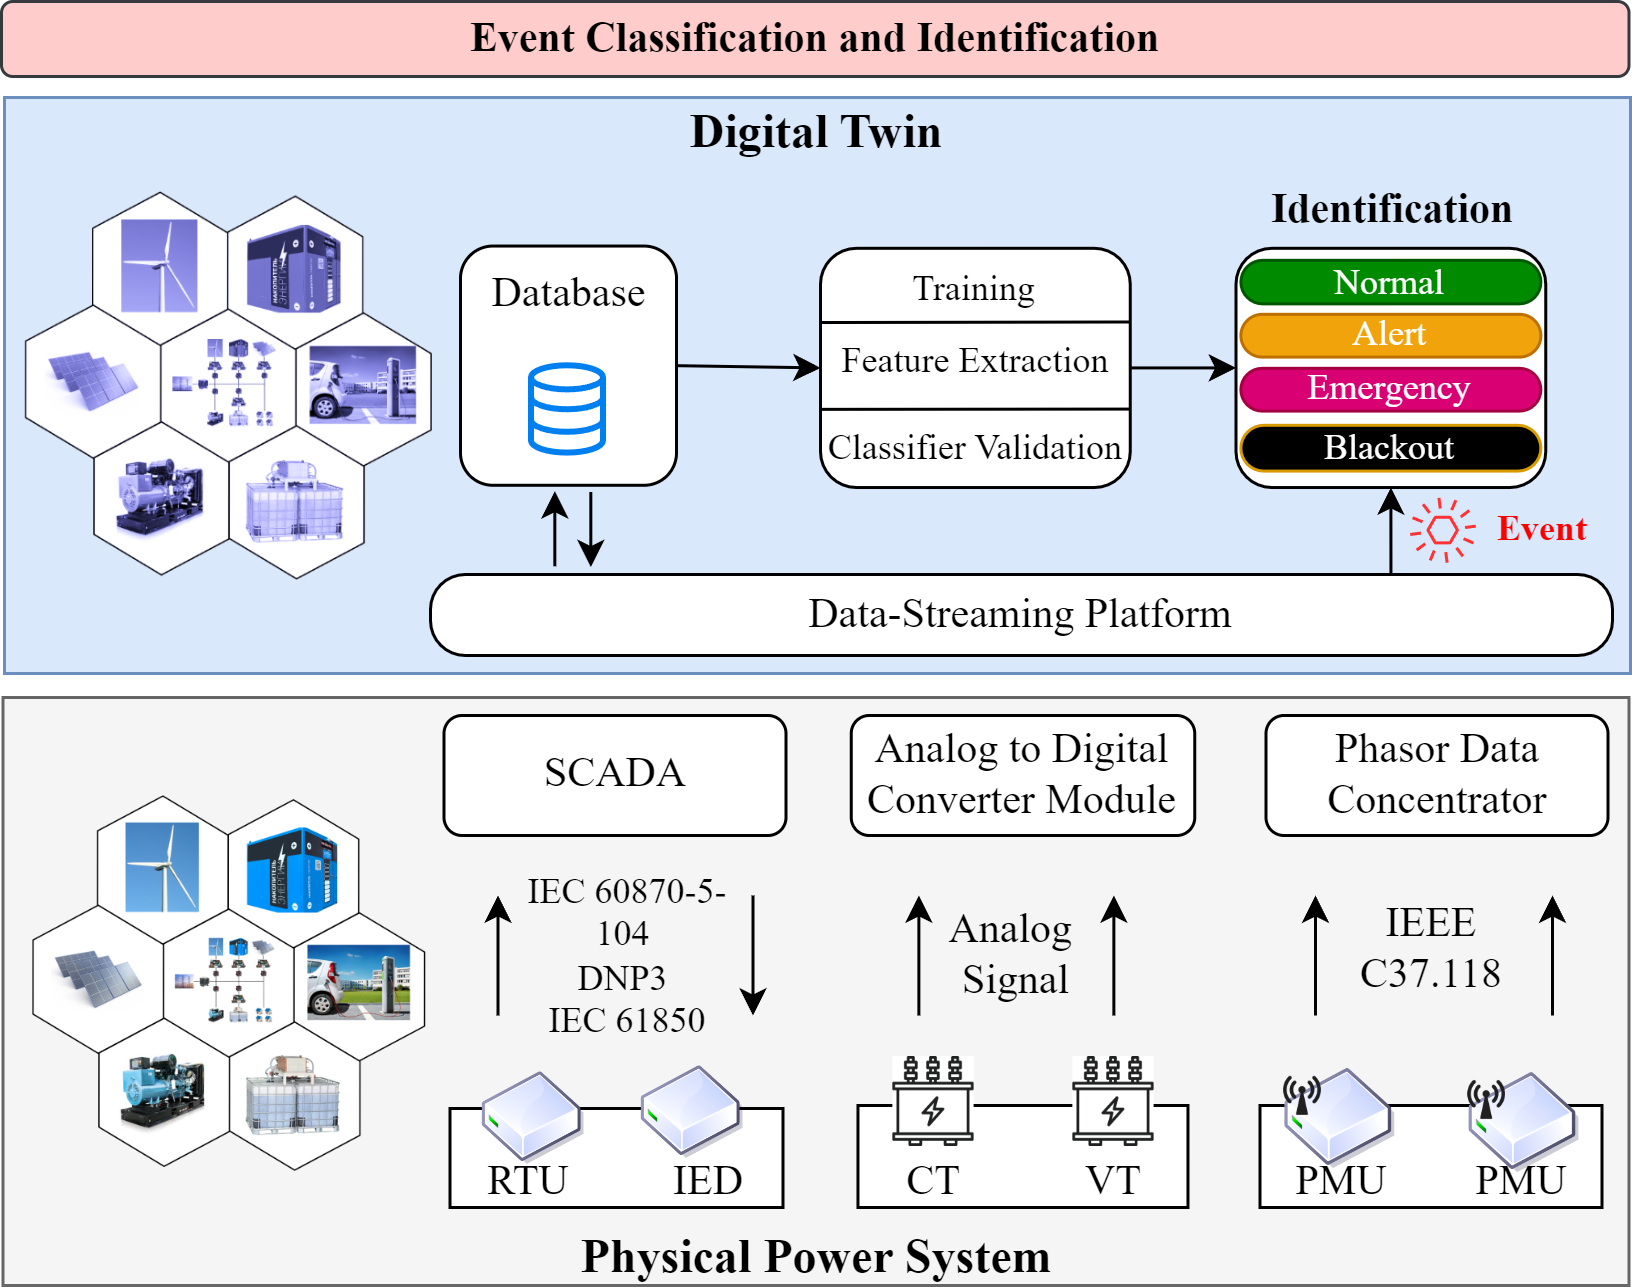
\includegraphics[scale=0.96]{dt_ml_idnt}
    }
    \caption{Classification and identification process of events based on DT and ML.}\label{fig:dt_ml_idnt}
\end{figure}

\subsection{Data Preprocessing}\label{subsec:ch2/sec3/sub1}

Data preprocessing is crucial to maintain its quality and ensure it is appropriate for modeling. The following steps were conducted:
\begin{enumerate}
    \item Data Cleaning: The raw data contained inconsistencies due to variations in data formats and potential errors during data collection. To address these issues, we first ensured accurate parsing of data by specifying the correct delimiter when importing the datasets. We standardized numerical values by replacing locale-specific decimal separators (e.g., commas) with periods. We then converted all numerical columns to appropriate data types to facilitate numerical computations. We identified and removed rows containing missing or invalid data entries to maintain data quality.
    \item Data Labeling: To prepare the data for supervised learning algorithms, we assigned binary labels to each data instance, with 0 indicating normal operation and 1 indicating an attack or anomaly. Then, we merged the labeled normal and attack datasets into a single cohesive dataset for subsequent analysis. To balance the impact of all features during the model training phase, feature scaling was applied as follows. We employed z-score normalization to transform the variables so their average is zero and their spread is standardized at one, defined as:
    \begin{equation}
        z=\frac{x-\mu}{\sigma},
    \end{equation}
    where $x$ is the value of the collected feature, $\mu$ is the feature mean, and $\sigma$ is the standard deviation.
\end{enumerate}

We conducted exploratory data analysis to gain insights into the characteristics of the data. We calculated descriptive statistics, including mean, median, variance, and interquartile ranges for each feature. We created time-series plots of power outputs and voltage levels to observe trends, patterns, and potential anomalies. Accordingly, we computed the Pearson correlation coefficients between features to identify multicollinearity, which could adversely affect certain modeling techniques.  We performed a feature selection to enhance model performance and interoperability by utilizing a Random Forest classifier to estimate feature importance based on the Gini impurity decrease criterion. The features have been ranked according to their importance scores to identify the most significant predictors influencing the target variable. We considered excluding features with low importance scores to reduce dimensionality and computational complexity without compromising model accuracy.

Given the potential imbalance between normal and attack instances in the dataset, we implemented techniques to address this issue. First, we augmented the dataset by introducing controlled Gaussian noise to the existing data points, thereby increasing variability and aiding the model in generalizing better. We utilized the Synthetic Minority Oversampling Technique (SMOTE) for artificial sample creation of the underrepresented class (attack data), weighing the class distribution and mitigating the risk of model bias towards the majority class. We randomized the order of data instances to eliminate any inherent order that could bias the model. The data was divided into separate training and testing subsets. using stratified sampling to preserve the original class proportions in both subsets.

\subsection{Traditional ML Approach}\label{subsec:ch2/sec3/sub2}
\begin{enumerate}
    \item Random Forest: First, a Random Forest \autocite{biau2015randomforestguidedtour} classifier was employed as a traditional ML model for anomaly detection. We defined settings, including the count of trees (estimators), the maximum depth a tree can grow, the minimum number of samples needed to split a node, and the minimum samples required at a leaf. We trained the model on the preprocessed and scaled training data. The training dataset enables the model to identify patterns and connections between the inputs and the target variable.

    \item Long Short-Term Memory (LSTM): An LSTM \autocite{Hochreiter_1997} architecture was utilized to capture temporal dependencies inherent in time-series data. We reshaped the dataset into sequences appropriate for LSTM input, with each sequence representing a time window of observations. The sequences and corresponding labels were converted into tensors compatible with the deep learning framework used for model implementation. We configured to accept input sequences of feature vectors. We included one or more LSTM layers to model sequential dependencies and retain information over time steps. A dense layer with appropriate activation (e.g., 4  sigmoid for binary classification) was added to produce the final output.
\end{enumerate}

We employed binary cross-entropy loss appropriate for our classification tasks. We used the Adam optimizer for efficient gradient descent. We carefully adjusted the learning rate, epochs, batch size, and hidden units to optimize model performance.  We assessed the model’s behavior on a validation set to monitor training progress and avoid overfitting. The final model was evaluated on the test set to attain a balanced estimate of its generalization. We applied k-fold crossvalidation to guarantee the strength of the outcomes and to mitigate the effects of any data partitioning bias. Where we first divided the dataset into k equally sized folds, repeatedly trained the model on k - 1 folds, and validated it on the remaining fold. We ensured that each fold maintained the same class distribution as the entire dataset to reflect the performance through various subsets accurately. The average and standard deviation of performance metrics are averaged across all folds to provide a comprehensive assessment.

Leveraging DT and ML techniques successfully demonstrates the synergistic potential of digital twin technology and machine learning for enhanced anomaly detection in power electronics-dominated grids. The DT provides a real-time, data-rich environment mirroring the physical system, enabling ML algorithms, specifically Random Forests and LSTMs, to learn normal operating patterns and identify subtle deviations indicative of cyberattacks or system faults.  Additionally, DT technology allows for training ML models with limited statistical data, leveraging its ability to simulate and generate robust datasets. DT not only a tool for performance enhancement but also a strategic enabler for effective threat detection in data-constrained environments. Future work should focus on optimizing model performance for higher grid dimensions to fully realize the potential of this method.